% \pagenumbering{arabic}
\Large
% \normalsize
\label{Chapter_2}
\section{Industrial IoT Security Landscape}
\label{sec:bg-landscape}

This section establishes the terrain on which this work is built. It defines the
Industrial Internet of Things and its mission-critical role, traces the evolution
that has led from isolated industrial control systems to the partitioned,
quantum-aware trust architectures examined here, characterises the scale of
deployment and the threat landscape it invites,  and reviews the regulatory
and standards context within which any deployable system must sit.
 
\subsection{From Industrial Control Systems to Trust-Partitioned IIoT}
\label{subsec:bg-evolution}
 
Industrial computing has passed through several distinct eras, and the security
problem addressed here is a product of that progression. Early industrial
control systems were isolated: programmable logic controllers and supervisory
systems operated on air-gapped networks, and security rested largely on physical
separation rather than on cryptography \cite{hussain2025survey}. The Industrial Internet of Things
dissolved that separation\cite{enemosah2024scada, kebande2024industrial}. By interconnecting sensors, controllers, actuators,
and gateways over shared networks, IIoT delivered real-time monitoring and
adaptive control, but it also exposed formerly isolated equipment to remote
adversaries\cite{kayan2022cybersecurity,zhukabayeva2025cybersecurity}. Subsequent phases layered artificial intelligence onto this fabric
for behavioural anomaly detection \cite{pinto2023survey, nuaimi2023intelligent}, and then introduced blockchain to provide
tamper-evident provenance for the data and decisions that AI produced \cite{amadi2026security,khan2022internet,huo2022comprehensive}. The
present phase, the one STRATA occupies, adds two further requirements: that trust
be partitioned across tiered ledgers so that heavyweight security work does not
fall on the weakest devices, and that the cryptography underpinning identity and
key exchange be resilient against an emerging quantum adversary.
Figure~\ref{fig:iiot-evolution} traces this progression and situates the present
contribution at its endpoint.


\begin{figure}[htbp]
    \centering
     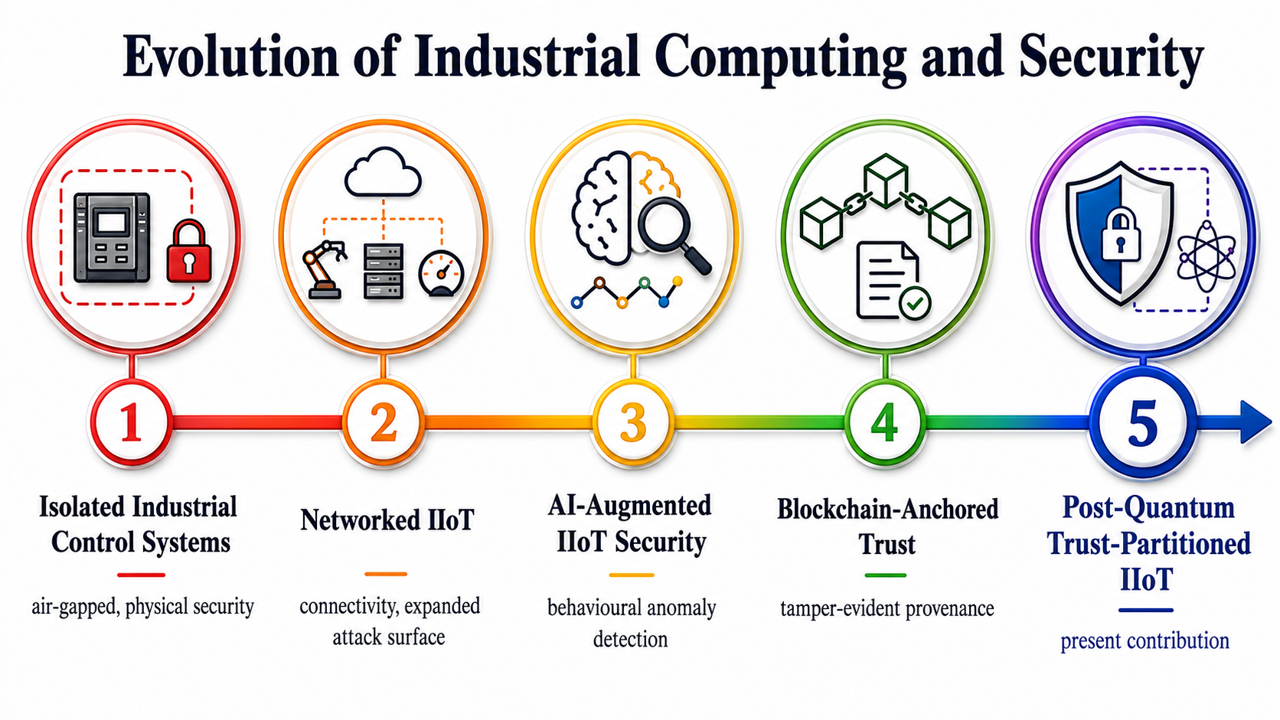
\includegraphics[width=0.95\textwidth]{figures/Picture2-evolution.png}
    \caption{Evolution of industrial computing security, from isolated control
    systems to post-quantum, trust-partitioned architecture.}
    \label{fig:iiot-evolution}
\end{figure}
 
\subsection{Scale and Mission-Critical Role}
\label{subsec:bg-scale}
 
The IIoT is now infrastructure at a scale that makes its security a matter of
public consequence rather than private inconvenience. The global installed base
of connected IoT devices reached approximately 18.5~billion in 2024 and is
projected to grow to 21.1~billion by the end of 2025 and to 39~billion by 2030,
a compound annual growth rate of about 13.2\%~\cite{iotanalytics2025}. The data
these devices generate grows in step with their number: IDC's Data Age 2025
study forecast that the global datasphere, the total volume of data created,
captured, and replicated worldwide each year, would expand from 45~zettabytes in
2019 to 175~zettabytes by 2025~\cite{idc_dataage2025}. A growing share of this
base is embedded in manufacturing, energy, water, and transportation systems,
where the data exchanged does not merely inform but directly actuates physical
processes. In such settings a corrupted reading, a forged command, or a delayed
validation is not a data-quality issue but a safety and continuity issue\cite{yu2023survey}, and
this is what distinguishes industrial security from its enterprise counterpart\cite{lehto2022cyber}.
Table~\ref{tab:iiot-stats} consolidates the scale, threat, and cost figures that
frame the problem, each drawn from its primary source.
 


\begin{table}[htbp]
\centering
\caption{Quantitative indicators motivating IIoT security: scale of deployment,
rise in attacks, cost of breaches, and cryptographic urgency.}
\label{tab:iiot-stats}
\small
\renewcommand{\arraystretch}{1.4}
\arrayrulecolor{red!70!black}
\begin{tabular}{@{}l r p{6.2cm}@{}}
\specialrule{1.2pt}{0pt}{0pt}
\rowcolor{red!12}
\textbf{Dimension} & \textbf{Quantity} & \textbf{Interpretation} \\
\specialrule{1.2pt}{0pt}{0pt}
\arrayrulecolor{black}
\textbf{Scale}
  & 18.5 $\rightarrow$ 39 billion
  & Connected IoT devices, 2024 to 2030 (projected), a 13.2\% compound annual growth rate. \\
\addlinespace
  & 175 ZB
  & Global data volume forecast for 2025. \\
\midrule
\textbf{Threat}
  & $+87\%$
  & Year-over-year rise in ransomware against industrial systems. \\
\addlinespace
  & $>50\%$
  & Share of ransomware victims in manufacturing. \\
\addlinespace
  & 25\%
  & Incidents forcing a full operational-technology shutdown. \\
\midrule
\textbf{Cost}
  & USD 4.44 M
  & Average cost of a data breach, global. \\
\addlinespace
  & USD 10.22 M
  & Average cost of a data breach, United States. \\
\midrule
\textbf{Urgency}
  & 2024
  & Post-quantum standards (FIPS 203/204/205) finalised, starting migration deadlines for current cryptography. \\
\arrayrulecolor{red!70!black}
\specialrule{1.2pt}{0pt}{0pt}
\arrayrulecolor{black}
\end{tabular}

\vspace{4pt}
{\footnotesize\itshape Sources: IoT Analytics (2025); IDC Data Age 2025;
Dragos (2025); IBM/Ponemon (2025); NIST (2024).}
\end{table}
 
\subsection{The Threat Landscape}
\label{subsec:bg-threats}
The consequence of pervasive connectivity is a substantially enlarged attack surface. Operational-technology environments, once peripheral to attacker interest, have become primary targets. Ransomware activity against industrial
organisations rose by more than 87\% year over year, the number of ransomware
groups directing effort at such organisations grew by 60\% to reach 80, and
manufacturing alone accounted for more than half of observed victims, with
roughly a quarter of incidents forcing a full shutdown of the affected
site~\cite{dragos2025}. The financial weight is of comparable order, the global
average cost of a data breach reaching USD~4.44~million and rising to
USD~10.22~million in the United States~\cite{ibm2025}. Beyond their headline
magnitude, these figures matter because industrial incidents convert directly
into physical disruption, which raises the stakes of every security decision at
the device level~\cite{yu2023survey}.

The specific forms these attacks take on industrial networks can be organised by
their traffic-level behaviour~\cite{aslam2024scrutinizing, sasi2024comprehensive}.
Denial-of-service and distributed denial-of-service attacks manifest as high-rate
flooding that saturates controllers and gateways; reconnaissance appears as
systematic probing of control-protocol ports; credential attacks show as
repeated authentication failures against brokers and controller interfaces; and
infiltration and botnet activity appear as anomalous payload entropy and periodic beaconing~\cite{gelgi2024systematic}. Table~\ref{tab:attack-map} maps these categories to their industrial manifestations, following the characterisation used in the behavioural detection work of Chapter~\ref{Chapter_4}.

\begin{table}[htbp]
\centering
\caption{Common attack categories and their manifestation in industrial network
traffic.}
\label{tab:attack-map}
\small
\begin{tabular}{p{3.0cm} p{4.5cm} p{5.0cm}}
\toprule
\textbf{Attack category} & \textbf{Traffic-level behaviour} & \textbf{Industrial manifestation} \\
\midrule
DoS / DDoS & High-rate flooding above normal baseline & Controller or gateway saturation, sensor jamming \\
Port scanning & Aggressive probing of many ports & Enumeration of control-protocol ports before intrusion \\
Brute force & Repeated authentication failures & Credential guessing against brokers and controller logins \\
Infiltration / malware & Elevated payload entropy, irregular flow sizes & Unauthorised firmware upload, code injection \\
Botnet / command-and-control & Periodic beaconing, low-entropy commands & Compromised devices in coordinated attacks \\
\bottomrule
\end{tabular}
\end{table}
 

\begin{figure}[htbp]
    \centering
     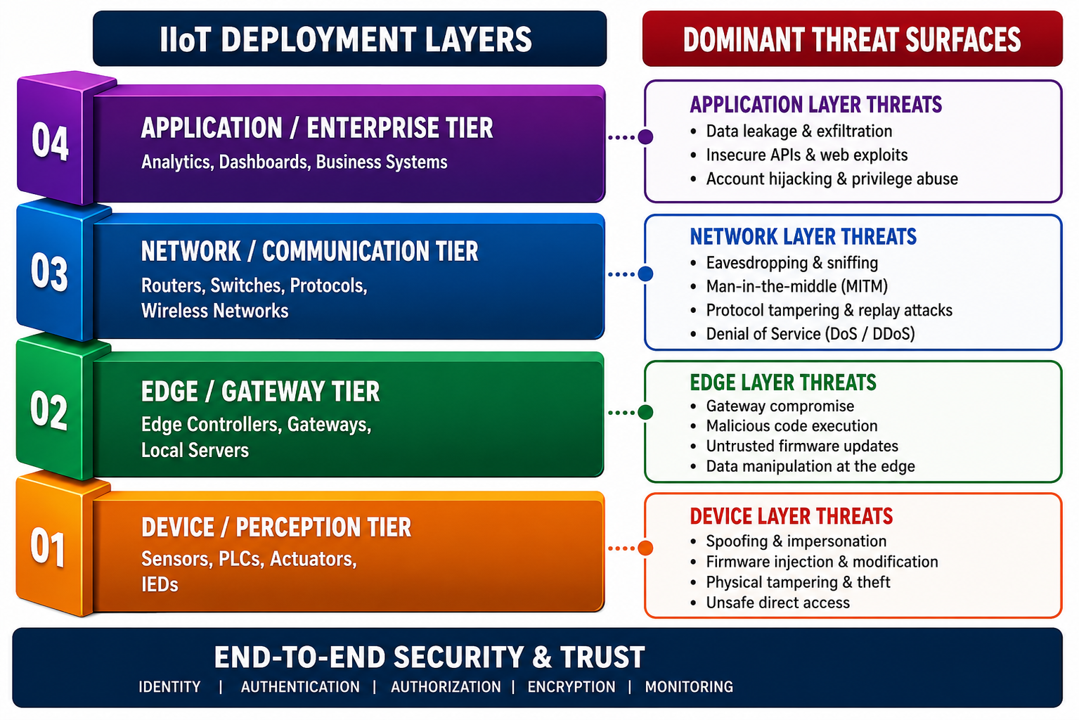
\includegraphics[width=0.95\textwidth]{figures/Picture3_threat.png}
    \caption{Layered view of an industrial IoT deployment and the dominant threat surface at each tier.}
    \label{fig:iiot-stack}
\end{figure}
 
\subsection{Regulatory and Standards Context}
\label{subsec:bg-regulatory}
Any deployable industrial security system sits within a regulatory and standards
environment that is itself evolving. The strategic value of industrial data
sharing is increasingly recognised in policy, with instruments such as the EU
Data Act of 2023 reflecting formal recognition of its
importance~\cite{stripped}. % TODO: replace `stripped` with the real EU Data Act entry from your DT paper's .bib

The cryptographic side of this environment has shifted even more sharply. The
asymmetric schemes that underpin current authentication and key exchange derive
their security from problems that a sufficiently capable quantum computer could
solve efficiently using Shor's algorithm~\cite{shor1999polynomial}. The risk is
not deferred to the arrival of such a machine: under the harvest-now,
decrypt-later model, an adversary can capture encrypted traffic today and decrypt
it once the capability matures, placing data with a long confidentiality horizon
at present risk~\cite{kagai2025harvest}. These pressures moved the quantum threat
from a research concern to a compliance one. In August 2024 the United States
National Institute of Standards and Technology finalised its first post-quantum
standards, FIPS 203, FIPS 204, and FIPS 205, concluding a process begun in
2016~\cite{fips203, fips204, fips205}.

The practical consequence for industrial deployment is that migration toward
quantum-resilient primitives is now an anticipated requirement rather than an
optional enhancement, and systems designed today are reasonably expected to
accommodate it~\cite{wang2025review}. The tension this creates for constrained
hardware, namely that post-quantum primitives carry larger keys and ciphertexts
than the schemes they replace and must be made to fit devices that are already
limited, is one of the motivating problems addressed in the chapters that
follow~\cite{fitzgibbon2024constrained}.



% ============================================================
% Chapter 2 — Section 2.2 (rich build)
% Learning-Based Security for Constrained IIoT
% Style: no em-dashes, no \emph, direct register (no "this thesis"/"we").
% Scope: MECHANISMS only. No measured results (params, accuracy, latency
% belong in Ch.4/5). Does NOT re-argue the constrained-hardware limits
% already covered in 2.1.4; here the focus is the learning methods.
%
% CITATION FLAGS: each [CITE: ...] marks a spot needing an external
% scholarly source, with a suggested Scholar search. Your own papers are
% cited with placeholder keys (amadi2026lightweight / amadi2026security /
% amadi2026identity) — confirm these match your .bib.
% ============================================================

\section{Learning-Based Security for Constrained IIoT}
\label{sec:bg-learning}

Signature-based and rule-based defences, which match traffic against catalogues
of known attack patterns, are poorly suited to industrial IoT. They cannot
recognise novel or zero-day behaviour, they require constant manual updating, and
their central deployment assumes a visibility over device traffic that
distributed industrial networks do not provide. Learning-based methods address
these gaps by modelling normal behaviour and flagging deviations from it, which
allows previously unseen attacks to be detected as anomalies rather than as known
signatures. This section explains the learning methods on which the systems in
this work rest: federated learning as the training paradigm, a hybrid
convolutional and recurrent network as the detection engine, and threshold-based
trust scoring as the mechanism that converts a detection into an enforceable
decision. The concern throughout is with how these methods operate; their
measured behaviour is reported in the evaluation.

\subsection{Federated Learning}
\label{subsec:bg-fl}

Conventional machine-learning pipelines are centralised: data is gathered from its
sources into a single repository where a model is trained. In distributed
industrial settings this arrangement is problematic on two counts. Transmitting
raw operational data to a central server consumes bandwidth that constrained
networks cannot spare, and it exposes sensitive process data to interception and
to privacy or confidentiality concerns\cite{lu2024federated,dritsas2025federated}.

Federated learning removes the need to centralise raw data. Each participating
device trains a local copy of a shared model on its own data and transmits only
the resulting model update, the adjusted parameters, to a coordinating
aggregator. The aggregator combines the updates from all participants into an
improved global model and returns it for the next round of local training. The
canonical aggregation rule, federated averaging, computes the global model as a
weighted average of the client updates, with each client weighted by the size of
its local dataset so that participants holding more data contribute
proportionally~\cite{amadi2026lightweight}. Because the raw data never leaves the
device on which it was generated, federated learning reduces both the
communication cost and the privacy exposure of collaborative training, which is
what makes it appropriate for distributed industrial deployments in which data is
sensitive and connectivity is limited\cite{ali2024blockchain}. Table~\ref{tab:central-vs-fl} contrasts the
two training paradigms across the dimensions that matter for constrained
industrial deployment.

\begin{table}[htbp]
\centering
\caption{Centralised and federated learning contrasted for distributed
industrial deployment.}
\label{tab:central-vs-fl}
\small
\renewcommand{\arraystretch}{1.3}
\begin{tabular}{@{}l l l@{}}
\toprule
\textbf{Aspect} & \textbf{Centralised learning} & \textbf{Federated learning} \\
\midrule
Location of raw data   & Moved to a central server      & Remains on the source device \\
Data transmitted       & Full raw datasets              & Model updates only \\
Privacy exposure       & High                           & Reduced \\
Communication cost     & High                           & Lower \\
Single point of failure& The central repository         & No shared raw-data store \\
Fit for constrained IIoT & Poor                         & Good \\
\bottomrule
\end{tabular}
\end{table}


\begin{figure}[htbp]
    \centering
    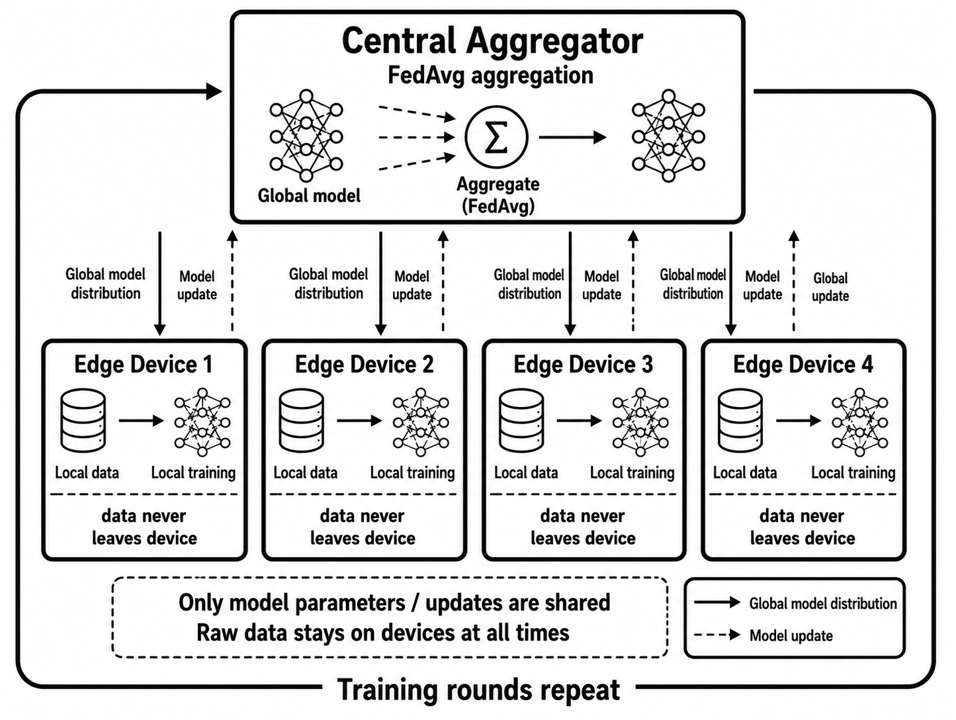
\includegraphics[width=0.95\textwidth]{figures/Picture4.png}
    \caption{Federated learning workflow. Devices train locally on data that
    never leaves the device and transmit only model updates, which the aggregator
    combines by federated averaging into an improved global model.}
    \label{fig:fl-workflow}
\end{figure}

Federated learning also aligns naturally with a tiered trust architecture. Local
model training occurs at or near the devices, while the aggregation and the
recording of accepted updates occur at a better-resourced tier, which mirrors the
separation between a fast device-facing layer and a coordinating layer developed
later in this work.

\subsection{Convolutional and Recurrent Modelling}
\label{subsec:bg-cnnlstm}
The detection engine used across the systems studied here is a hybrid network
that combines a one-dimensional convolutional stage with a recurrent stage. The
design is motivated by the structure of industrial network traffic, which is a
sequence of flow records exhibiting two kinds of pattern at once. There are
short-range, local patterns, such as burst rates, packet-size distributions, and
protocol-flag combinations, and there are longer-range temporal dependencies
arising from periodic sensing, control loops, and attack behaviour that unfolds
over time.

A one-dimensional convolutional layer is well suited to the first kind. It slides
learnable filters across the feature sequence and extracts local patterns
efficiently, producing feature maps that summarise the salient short-range
structure of the input~\cite{ige2024state, arsalan20241d}. A pooling stage then
reduces the dimensionality of these feature maps, retaining the strongest
responses while discarding fine-grained detail, which lowers computational cost
and improves robustness to small shifts in the input. The convolutional and
pooling stages together act as a feature compressor, reducing the raw input to a
compact set of representative features.
This compressed representation has, however, no explicit memory of order beyond
the span of the filters. A recurrent layer supplies that memory. A Long
Short-Term Memory network processes the sequence step by step and maintains an
internal state through gated connections that allow it to retain relevant
information across long spans while discarding the irrelevant, which lets it
model dependencies that a convolutional layer alone cannot~\cite{krichen2025long}.

Placing these stages in sequence, convolutional feature extraction and pooling
followed by recurrent temporal modelling, produces an engine that captures both
the local signatures and the temporal evolution of industrial
traffic~\cite{bamber2025hybrid}, with a final classification stage mapping the
learned representation to a probability over the traffic
classes~\cite{amadi2026lightweight, amadi2026security}. This
convolutional-recurrent pairing is the behavioural engine common to the systems
examined in the later chapters. Figure~\ref{fig:cnn-lstm} shows the arrangement
of stages, and Table~\ref{tab:cnn-lstm-stages} summarises the function of each.
\begin{figure}[htbp]
    \centering
    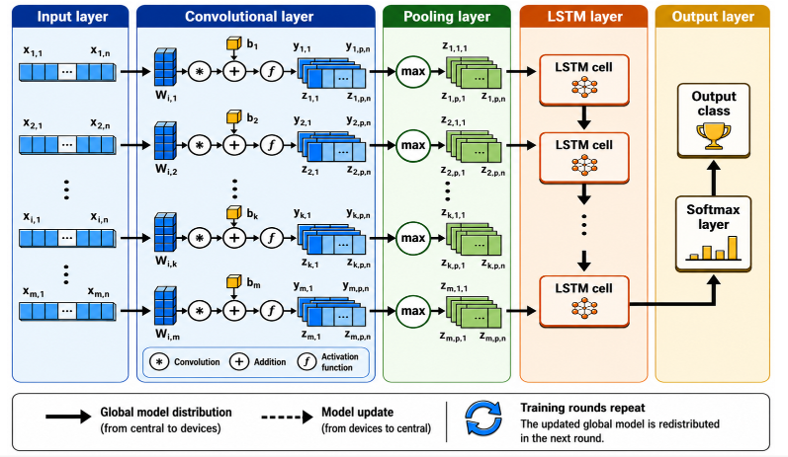
\includegraphics[width=0.89\textwidth]{figures/Picture5.png}
    \caption{Hybrid one-dimensional convolutional and recurrent detection engine.
    Convolutional and pooling layers extract and compress local features from the
    traffic sequence, the recurrent layer models temporal dependence, and a
    classification stage produces class probabilities.}
    \label{fig:cnn-lstm}
\end{figure}

\begin{table}[htbp]
\centering
\caption{Function of each stage in the hybrid convolutional-recurrent detection
engine.}
\label{tab:cnn-lstm-stages}
\small
\renewcommand{\arraystretch}{1.3}
\begin{tabular}{@{}l p{9cm}@{}}
\toprule
\textbf{Stage} & \textbf{Function} \\
\midrule
Input          & Receives the ordered sequence of network-flow features. \\
1D convolution & Extracts short-range local patterns from the feature sequence. \\
Pooling        & Reduces the dimensionality of the feature maps, retaining the strongest responses and improving robustness. \\
Recurrent (LSTM) & Models longer-range temporal dependencies across the sequence through gated memory. \\
Classification & Maps the learned representation to a probability over the traffic classes. \\
\bottomrule
\end{tabular}
\end{table}
The same architectural family appears in more than one system, instantiated on
different data. In one system it is trained on a network-intrusion benchmark and
discriminates among five traffic classes covering denial-of-service, probing,
unauthorised-access, and normal categories~\cite{amadi2026security}; in another
it is trained on a fused intrusion-detection collection and discriminates among
eight classes covering seven attack categories and one benign
class~\cite{amadi2026lightweight}. The two instances share the
convolutional-recurrent structure while differing in their datasets and their
class sets. This common lineage is noted because it recurs in the architecture
developed later.

\subsection{Trust Scoring and Revocation}
\label{subsec:bg-trust}

Detection is only useful if it drives an action. Behavioural trust management, in
which a node's trustworthiness is quantified from its observed behaviour and used
to govern its participation, is an established response to the problem of
malicious or compromised nodes in distributed and industrial
networks~\cite{ferraris2024survey}. Rather than treating security as a single
admitted-or-blocked decision made once at authentication, such schemes maintain a
continuous, evolving measure of each node's reliability and adjust it as
behaviour is observed~\cite{ullah2024deep}.

In the systems studied here, this principle is realised through a defined
sequence, illustrated in Figure~\ref{fig:trust-flow}. The behavioural engine
produces, for the device or node whose traffic was classified, a set of class
probabilities across normal and anomalous categories. These are reduced to a
single trust score in the range $[0,1]$, which is then compared against a
predefined threshold $\tau$. A device whose score satisfies $\text{score} \geq
\tau$ is treated as trustworthy and its interactions proceed; a device whose
score falls below the threshold, $\text{score} < \tau$, is flagged as anomalous.
Threshold-based conversion of a continuous anomaly signal into a discrete
security decision of this kind is a common and well-studied mechanism in network
anomaly detection~\cite{komadina2024comparing}.

A flagged device is not merely logged. It is moved through a defined lifecycle
toward isolation, in which its interactions are restricted or quarantined, and
its revocation is then recorded so that other participants no longer extend trust
to it. Anchoring trust and revocation decisions on a distributed ledger is a
recognised approach to making them tamper-evident and consistent across a
decentralised network, since no single participant can unilaterally reinstate a
revoked node~\cite{d2025blockchain}. Once the revocation is written as an
immutable ledger record, the event is propagated to the other nodes, which update
their trust state accordingly. In the present systems, this ledger-recorded and
broadcast revocation is what prevents a node excluded at one point from silently
re-entering elsewhere~\cite{amadi2026symmetric}. This coupling, from
class-probability output, to a trust score, to a threshold comparison, and then
to a ledger-recorded and propagated revocation, is the mechanism by which
learning-based detection becomes an enforceable trust decision.
Table~\ref{tab:trust-stages} summarises the role of each stage.

\begin{figure}[htbp]
    \centering
     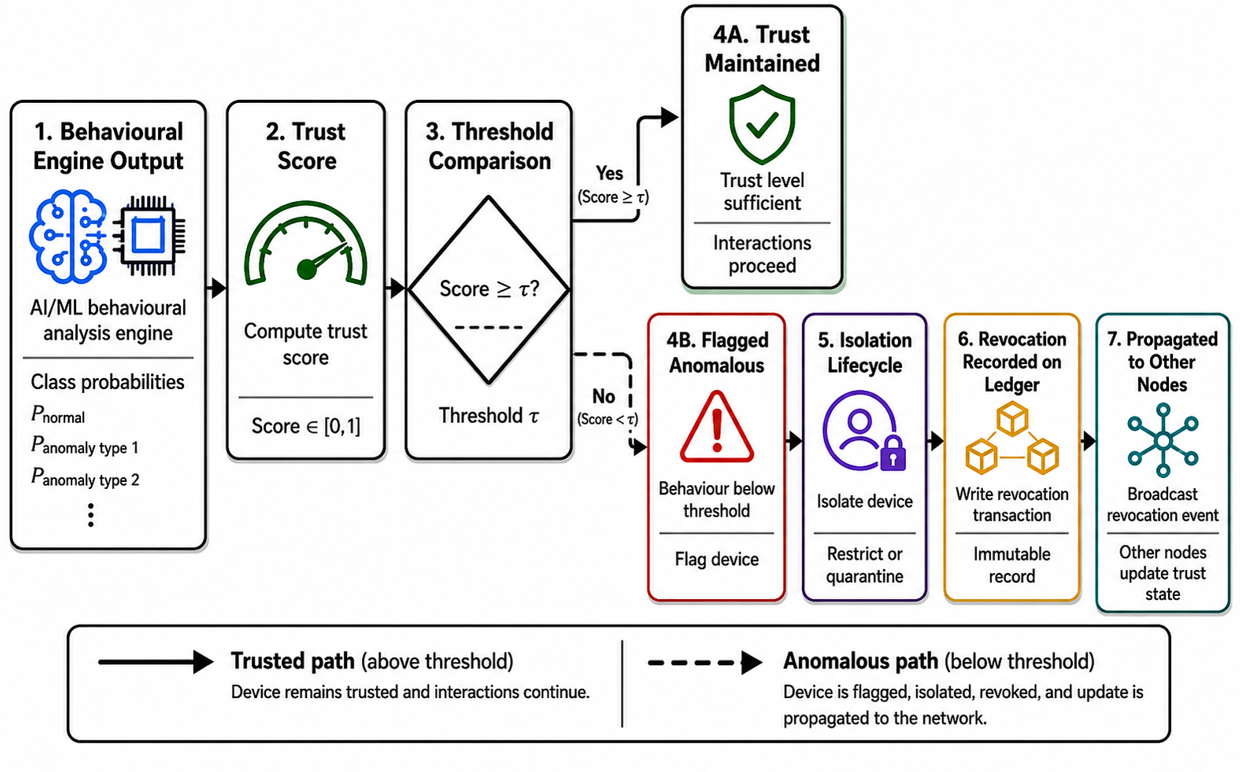
\includegraphics[width=1.05\textwidth]{figures/Picture62.PNG}
    \caption{From Detection to Enforcement: The behavioural engine's class
    probabilities yield a trust score, which is compared against the threshold $\tau$. A device with score at or above $\tau$ retains trust and its interactions proceed; a device below $\tau$ is flagged, isolated, has its revocation recorded as an immutable ledger record, and has that revocation propagated to the other nodes.}
    \label{fig:trust-flow}
\end{figure}

\begin{table}[htbp]
\centering
\caption{Stages in the trust-scoring and revocation mechanism.}
\label{tab:trust-stages}
\small
\renewcommand{\arraystretch}{1.3}
\begin{tabular}{@{}l p{8.8cm}@{}}
\toprule
\textbf{Stage} & \textbf{Function} \\
\midrule
Behavioural engine output & Produces class probabilities across normal and anomalous categories for the classified node. \\
Trust score               & Reduces the class probabilities to a single trust score in $[0,1]$. \\
Threshold comparison      & Compares the score against the threshold $\tau$ to yield a trust or anomaly verdict. \\
Trust maintained          & For a score at or above $\tau$, the device stays trusted and its interactions proceed. \\
Flagging and isolation    & For a score below $\tau$, the device is flagged anomalous and moved through an isolation lifecycle. \\
Revocation                & Writes the revocation as an immutable ledger record, making it tamper-evident. \\
Propagation               & Broadcasts the revocation so other nodes update their trust state and the device cannot re-enter elsewhere. \\
\bottomrule
\end{tabular}
\end{table}

The trust-scoring mechanism connects the learning methods of this section to the
ledger mechanisms that follow. The behavioural engine produces the evidence, the
threshold turns that evidence into a verdict, and the ledger gives the verdict
durability and reach. It is this chain, rather than any single component, that
constitutes the learning-based security foundation on which the proposed
architecture is built.




\section{AI Models and Cognitive Engines for IIoT Security}
\label{sec:ai-models}
 
From the foregoing analysis, protecting constrained, mission-critical IIoT against the threat landscape of Section~\ref{sec:bg-landscape} rests not only on the learning-based mechanisms of Section~\ref{sec:bg-learning} but on the model family that underpins them. An artificial intelligence model in this setting is a function learned from data that maps device and network observations to a security decision, and the cognitive engine is that trained model together with the calibration and scoring logic that turns its raw output into a usable, thresholded verdict. The model family is decisive, because each family carries a distinct inductive bias, data appetite, and transparency profile that fixes both what the engine can detect and how far its decision can be trusted and audited. A margin-based classifier, a convolutional feature extractor, and a graph model differ not merely in accuracy but in whether their outputs are interpretable, whether their probabilities can be calibrated, and whether their execution can be reproduced for audit. Those differences weigh most heavily under the resource and trust budget of an industrial device, where a model that cannot run within the device envelope, or whose decision cannot be reconstructed, is unsuitable however strong its benchmark accuracy.

\begin{figure}[t]
  \centering
   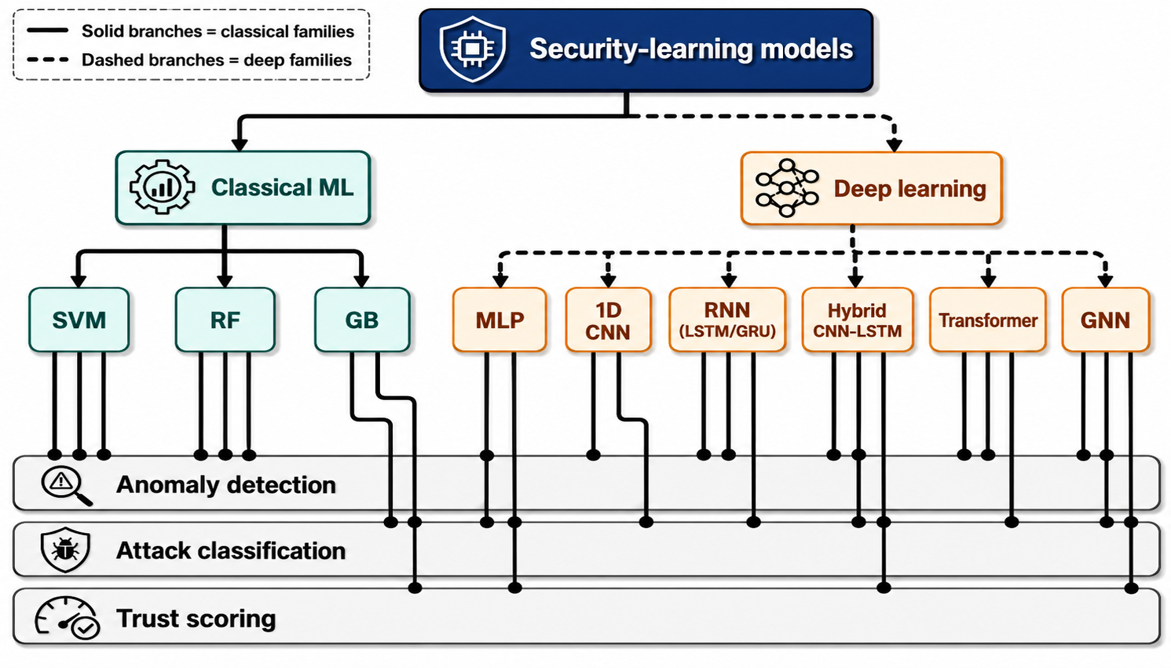
\includegraphics[width=\textwidth]{figures/Picture7.png}
  \caption{Taxonomy of AI model families for IIoT security, grouped by representational depth and mapped to the security-learning tasks each serves.}
 \label{fig:ai-taxonomy}
\end{figure}

\subsection{Model Families and the Security-Learning Tasks}
\label{subsec:model-taxonomy}
 Security learning in IIoT reduces to a small set of canonical tasks: binary anomaly detection, which separates normal from abnormal behaviour; multi-class attack classification, which assigns an observation to a specific attack category; and continuous behavioural trust scoring, which maps a device or flow to a graded reliability value. Sequential and topology-aware variants extend these tasks to telemetry that carries temporal or relational structure. Comprehensive surveys of machine-learning and deep-learning intrusion detection organise the field along these lines, cataloguing the algorithms, datasets, and attack categories that recur across deployments \cite{ali2024unveiling,kikissagbe2024machine}. A consistent finding across them is that each task admits treatment by more than one model family, so family selection is a design decision rather than a fixed consequence of the task.

\begin{table}[htbp]
  \centering
  \footnotesize
  \setlength{\tabcolsep}{4pt}
  \renewcommand{\arraystretch}{1.25}
  \caption{AI model families for IIoT security compared across the dimensions that govern trustworthy deployment. Entries are family-level properties, not measured results.}
  \label{tab:ai-family-comparison}
  \begin{tabularx}{\textwidth}{@{}
      >{\raggedright\arraybackslash}p{2.4cm}
      >{\raggedright\arraybackslash}X
      >{\raggedright\arraybackslash}X
      >{\raggedright\arraybackslash}X
      >{\raggedright\arraybackslash}X
      >{\raggedright\arraybackslash}p{1.6cm}@{}}
    \toprule
    \textbf{Model family} & \textbf{Typical role} & \textbf{Key strength} & \textbf{Key limitation} & \textbf{Transparency / trust} & \textbf{Device fit} \\
    \midrule
    Classical ML (SVM, RF, GB) & Tabular / flow anomaly and attack classification & Data-efficient; strong on engineered features; deterministic & Manual features; no native spatial or temporal modelling & High: interpretable, calibratable, reproducible & Good \\
    \addlinespace
    MLP & Nonlinear classification over features & Captures higher-order feature interactions & No structural prior; data-hungry; opaque & Low; calibratable & Moderate \\
    \addlinespace
    1D CNN & Local pattern extraction from flow or payload sequences & Parameter-efficient; translation-invariant local features & Limited long-range temporal context & Low; saliency gives partial insight & Moderate \\
    \addlinespace
    RNN / LSTM / GRU & Temporal telemetry; attack progression & Models long-range temporal dependencies & Sequential compute; hard to parallelise & Low; opaque gating & Moderate to poor \\
    \addlinespace
    Hybrid CNN-LSTM & Joint spatial-temporal behavioural detection & Combines local extraction with temporal modelling & Higher parameter and compute cost & Low; needs post-hoc XAI and calibration & Moderate \\
    \addlinespace
    Transformer / attention & Long-sequence dependency modelling & Global context; no recurrent bottleneck & Quadratic attention cost; large models & Attention gives partial insight & Poor unless offloaded \\
    \addlinespace
    GNN & Topology-aware detection (lateral movement, structure) & Encodes relational network structure & Graph construction and message-passing overhead & Low; graph explainability emerging & Poor to moderate \\
    \bottomrule
  \end{tabularx}
\end{table}

Two axes organise the family space. The first is representational depth: shallow, or classical, models operate on engineered features, whereas deep models learn representations directly from raw or lightly processed inputs. The second is the structure of the input: tabular flow statistics suit feature-based classifiers, while raw packet, byte, or event sequences reward models with spatial or temporal priors. Recent reviews of machine-learning intrusion detection for the Internet of Things adopt a comparable organisation, grouping methods by learning paradigm and by the representation each consumes \cite{manivannan2024recent}. Figure~\ref{fig:ai-taxonomy} maps the families reviewed here onto the tasks they serve, and Table~\ref{tab:ai-family-comparison} compares them across the dimensions that matter for industrial deployment.

 
The IIoT setting imposes a third axis that general machine-learning benchmarks omit: the resource and trust budget. A model that cannot execute within a Class~1 device budget, or whose outputs cannot be calibrated and audited, is unsuitable for mission-critical use, however high its benchmark accuracy. Comparative evaluations of lightweight classifiers across IoT and industrial IoT datasets show that detection quality and resource cost trade against one another, so the technique that ranks first on accuracy is rarely the one that fits the device \cite{ismail2025intrusion}, and edge-oriented designs recover deployability only through explicit optimisation such as feature reduction and model quantisation \cite{tiwari2024lightweight}. Surveys of security for resource-constrained devices treat this budget as a primary design constraint rather than a secondary concern \cite{altaibek2025survey}. This axis reweights the comparison throughout the section, favouring families whose cost and transparency remain within reach of the device rather than those that maximise raw discriminative power alone.

\subsection{Classical Machine Learning}
\label{subsec:classical-ml}
Support vector machines separate classes by the maximum-margin hyperplane in a feature space that a kernel makes implicitly nonlinear. The margin formulation performs well in high-dimensional feature spaces and captures nonlinear attack patterns through the kernel, which has made it a recurring choice for intrusion detection in the Internet of Things \cite{sama2024cutting}. Fine-tuned linear and feature-selected variants deliver accurate detection at a small model size well matched to constrained gateways \cite{azimjonov2024designing}, and hybrid rule-augmented designs extend the approach to heterogeneous IoT threat data \cite{ashraf2024hybrid}. The principal limitation is scalability: kernel training scales quadratically in the number of samples, so large corpora require dimensionality reduction or optimisation of the support-vector search to remain tractable \cite{raghunath2025pca}. Because the decision boundary depends only on a compact set of support vectors, the trained model itself remains small, which is an advantage on resource-limited hardware.
 
Tree ensembles occupy the opposite end of the classical spectrum. Random forests aggregate many decorrelated decision trees by bagging, while gradient boosting builds trees sequentially to correct the residual error of the ensemble so far. Both handle heterogeneous tabular flow features with minimal preprocessing and deliver strong performance out of the box, and lightweight tree-based detectors are for this reason widely deployed on resource-constrained IoT nodes where preprocessing and compute headroom are scarce \cite{mishra2025lirad,pandey2025lightweight}. Their split structure also yields native feature-importance measures, so an analyst can trace which features drove a decision.
 
Three properties shared across the classical family bear directly on trust. Classical models are data-efficient, deterministic under fixed seeds, and interpretable, since tree paths and linear or margin weights expose the basis of a decision \cite{abdelaziz2025enhancing}. Determinism in particular makes their outputs reproducible and therefore auditable, a property that Section~\ref{subsec:transparency-trust} develops as a trust requirement. The countervailing limitation is that classical models depend on manual feature engineering and do not natively represent the spatial or temporal structure present in raw traffic, which motivates the deep architectures reviewed next.
% ---------------------------------------------------------------------
\subsection{Deep Learning Architectures}
\label{subsec:deep-learning}
 
The multilayer perceptron is the deep baseline. Stacked nonlinear layers approximate arbitrary functions over engineered features and capture higher-order feature interactions beyond the reach of linear models, but the absence of any structural prior makes the perceptron data-hungry and its learned weights opaque \cite{cherfi2025mlp,zhao2025research}. It improves discriminative power at a direct cost in interpretability.
 
Convolutional networks introduce a spatial prior. Applied in one dimension over packet, byte, or flow sequences, convolutional filters extract local patterns through weight sharing and translation invariance, which yields parameter efficiency relative to a fully connected network of comparable capacity \cite{kumar2024deep}. The trade is a limited receptive field, so local motifs are captured well but long-range temporal context is not. Recurrent networks supply that missing temporal prior: gated variants, principally the long short-term memory and gated recurrent unit, model long-range dependencies across event sequences and so capture the progression of an attack over time, at the cost of sequential computation that resists parallelisation \cite{devendiran2024dugat}. Hybrid convolutional-recurrent models compose the two priors, placing convolutional feature extraction ahead of recurrent temporal modelling so that local structure and temporal dependency are learned jointly \cite{psychogyios2024deep}.
 
Two further families extend the design space at higher cost. Attention-based transformers replace recurrence with self-attention, modelling global dependencies across a sequence without a recurrent bottleneck and performing strongly on long inputs, but the quadratic cost of attention and the large parameter counts of these models strain constrained device budgets unless inference is offloaded \cite{ali2024empowering}. Graph neural networks encode the network as a graph of devices and flows and learn topology-aware embeddings, which suit the detection of lateral movement and structural anomalies that feature-based models miss. However, graph construction and message passing add their own overhead \cite{xu2024applying,zhong2024survey} Table~\ref{tab:task-family-fit} summarizes which families best serve each security task.
 
\begin{table}[t]
  \centering
  \caption{Security-learning tasks and the model families best suited to each.}
  \label{tab:task-family-fit}
  \renewcommand{\arraystretch}{1.3}
  \begin{tabularx}{\columnwidth}{@{}l >{\raggedright\arraybackslash}X@{}}
    \toprule
    \textbf{Security-learning task} & \textbf{Best-suited families} \\
    \midrule
    Binary anomaly detection (tabular flow)   & Classical ML; MLP \\
    Multi-class attack classification          & Tree ensembles; 1D CNN; hybrid CNN-LSTM \\
    Behavioural trust scoring (calibrated)     & Calibrated classical ML; hybrid CNN-LSTM with calibration \\
    Sequential / temporal detection            & LSTM / GRU; hybrid CNN-LSTM; transformer \\
    Topology-aware detection                   & GNN \\
    \bottomrule
  \end{tabularx}
\end{table}
 
\subsection{Transparency, Trust, and Reproducibility}
\label{subsec:transparency-trust}
Detection capability is necessary but not sufficient for trustworthy security. A recurring tension runs through the families above: representational power and transparency trade against each other, so the deep architectures that detect the subtlest attacks are also the least able to explain their alerts, while the classical models that explain themselves readily are the least expressive \cite{sharma2024explainable,mohale2025systematic}. 
Figure~\ref{fig:interpretability-tradeoff}
places the model families of this section on the interpretability capacity plane,
where the classical families occupy the high-transparency region compatible with
constrained, auditable deployment and the deep families trade that transparency for
representational power. 
Explainability methods partially close this gap for deep models. Post-hoc attribution such as feature-importance scoring and local surrogate explanation, together with attention inspection, recovers an approximate account of which inputs drove a prediction, but these explanations are estimates rather than the model's own reasoning and can be unstable across similar inputs \cite{gaspar2024explainable, wali2025explainable}. Transparency obtained this way is therefore a mitigation, not a substitute for an inherently interpretable model.

\begin{figure}[t]
  \centering
   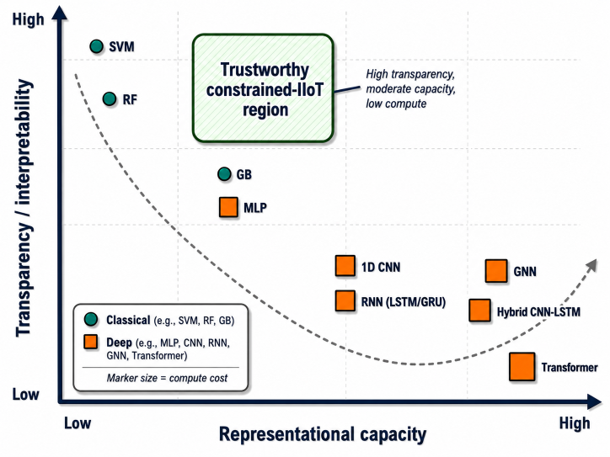
\includegraphics[width=1.05\columnwidth]{figures/Picture8.png}
 \caption{Interpretability against representational capacity for the model families of Section~\ref{sec:ai-models}. Classical families (circles) combine high transparency with moderate capacity and fall within the hatched envelope of trustworthy, auditable detection on constrained devices; deep families (squares) gain capacity at the cost of transparency and fall outside it.}
  \label{fig:interpretability-tradeoff}
\end{figure}
 
A second, distinct trust property is calibration. Behavioural trust scoring requires that a score behave as a faithful probability and not merely as a ranking, so that a fixed threshold carries a consistent meaning across devices and over time. Deep classifiers are frequently overconfident and require an explicit calibration step, such as isotonic or temperature scaling, before their outputs can support a principled threshold \cite{balanya2024adaptive, dong2025survey}. 
 
The final property is reproducibility. A security decision that cannot be reproduced cannot be independently audited, and reproducibility is far harder to guarantee for accelerated deep-learning pipelines, whose floating-point reduction orders vary across hardware, than for deterministic classical pipelines that yield bitwise-identical outputs under a fixed environment \cite{semmelrock2025reproducibility, kapoor2024reforms}. This reproducibility requirement, rather than raw accuracy alone, shapes the model choices that make verifiable IIoT security possible.
 

\section{Blockchain and Distributed Ledgers for IIoT}
\label{sec:blockchain-ledgers}
From the foregoing analysis, the behavioural trust decisions produced by the learning engines of Section~\ref{sec:ai-models} are only as dependable as the record that preserves them: a trust score, an alert, or a revocation event that can be altered after the fact cannot support accountable, auditable security in a mission-critical setting. A distributed ledger supplies that record. A blockchain is a distributed, append-only ledger in which transactions are grouped into blocks, and each block is bound to its predecessor by a cryptographic hash, so that any later modification is exposed by recomputation rather than concealed behind trust in a custodian \cite{xu2024exploring,savadatti2025survey}. The property that matters for constrained industrial deployments is not currency or decentralised finance but tamper-evident provenance: an immutable, independently checkable trail of the security-relevant events that a regulator or a partner institution must be able to reconstruct. Realising that property within a real device budget depends on three design choices, namely how the ledger is structured, who is permitted to write to it, and how distributed validators agree on its contents.


\subsection{Blocks, Hashing, and Immutability}
\label{subsec:blocks-hashing}
A block is a batch of transactions preceded by a header that records, among other fields, the cryptographic hash of the previous block. Chaining blocks by hash makes the ledger tamper-evident: altering any committed transaction changes its block hash, which invalidates the reference held by every subsequent block, so a single edit is detectable by recomputing the chain \cite{kuznetsov2024merkle}. Within a block, the transactions are summarised by a Merkle tree whose root commits to the entire set, allowing the membership of one transaction to be proven in logarithmic time without transmitting the whole block. Immutability is therefore a joint property of hash-linking and replication: the more independent validators that hold and verify the chain, the harder it becomes to rewrite history unilaterally, and the cheaper it is for any party to detect an attempt.
 
For constrained IIoT the cost of this guarantee is the binding concern. Full replication and continuous verification exceed the memory and energy budgets of low-class devices, and storing raw industrial payloads on-chain is infeasible at operational data rates. The standard resolution is to keep payloads off-chain and commit only their cryptographic digests to the ledger, so that integrity is certified without the ledger bearing the data volume \cite{eren2025security}.
 
\subsection{Permissioned and Permissionless Ledgers, and Smart Contracts}
\label{subsec:permissioned-contracts}
Ledgers differ in who may append to them. A permissionless ledger admits anonymous participants and resists censorship, but it pays for open membership with limited throughput and probabilistic finality, in which a committed block is only ever overwhelmingly, never certainly, final. A permissioned ledger restricts write access to a vetted set of validators, which yields higher throughput and deterministic finality at the cost of a narrower trust base. For constrained, mission-critical IIoT, the permissioned model is the natural fit, because an industrial consortium has identifiable members, contractual accountability, and regulatory obligations that an anonymous network cannot satisfy, and because deterministic finality aligns with the timing guarantees such systems require\cite{lahbib2024blockchain,bobde2024enhancing}.
 
Smart contracts extend a ledger from a passive record into an active policy layer. A smart contract is self-executing code stored on-chain and run identically by every validator, so its outcome is deterministic and independently verifiable rather than dependent on any single party \cite{wu2024comprehensive,wei2024survey}. This is the mechanism by which the behavioural policies such as a trust threshold, a revocation rule, or an access decision can be enforced on-chain: the same logic that scores a device can be encoded as contract logic that records, and acts on, the resulting verdict without a trusted intermediary. The contract does not improve the accuracy of the decision; it makes the decision and its consequences auditable.
 
\subsection{Consensus Families under Resource Constraints}
\label{subsec:consensus-families}
Consensus is the mechanism by which distributed validators agree on a single canonical ledger state despite faults and adversaries, and the families in use differ sharply in cost and finality. Proof-of-Work secures agreement through a computational puzzle and offers only probabilistic finality at very high energy cost. Proof-of-Stake replaces computation with economic stake, which lowers energy demand but presupposes a token economy. The Byzantine-fault-tolerant family, exemplified by Practical Byzantine Fault Tolerance, delivers deterministic finality and tolerates a bounded fraction of Byzantine validators, but its all-to-all messaging scales quadratically and so limits the practical validator-set size. Proof-of-Authority dispenses with both puzzles and stake: a small set of vetted authorities produce blocks in a fixed or rotating order, achieving deterministic finality at negligible energy cost~\cite{jain2025survey}. Table~\ref{tab:consensus-comparison} sets these families side by side on membership, finality, and fitness for a constrained industrial ledger, and shows why the choice narrows toward authority-based consensus once energy cost and deterministic finality are treated as hard requirements rather than preferences.

\begin{table}[t]
  \centering
  \footnotesize
  \setlength{\tabcolsep}{4pt}
  \renewcommand{\arraystretch}{1.25}
  \caption{Consensus families against the constraints of a permissioned industrial ledger. Entries are inherent mechanism properties, not measured results.}
  \label{tab:consensus-comparison}
  \begin{tabularx}{\columnwidth}{@{}
      >{\raggedright\arraybackslash}p{3.0cm}
      >{\raggedright\arraybackslash}p{2.1cm}
      >{\raggedright\arraybackslash}p{2.4cm}
      >{\raggedright\arraybackslash}X@{}}
    \toprule
    \textbf{Mechanism} & \textbf{Membership} & \textbf{Finality} & \textbf{Fit for constrained IIoT} \\
    \midrule
    Proof-of-Work                      & Permissionless & Probabilistic                  & Unsuitable; energy budget alone rules it out \\
    \addlinespace
    Proof-of-Stake                     & Permissionless & Near-final (variant-dependent) & Limited; presumes a token economy \\
    \addlinespace
    PBFT (BFT family)                  & Permissioned   & Deterministic                  & Small validator sets only (quadratic messaging) \\
    \addlinespace
    Proof-of-Authority                 & Permissioned   & Deterministic                  & Well suited to closed consortia \\
    \addlinespace
    Proof-of-Authority-and-Association & Permissioned   & Deterministic                  & Adds reliability-weighted, self-healing validators \\
    \bottomrule
  \end{tabularx}
\end{table}
The implications for constrained IIoT are direct. The computational puzzle of Proof-of-Work is categorically incompatible with low-class energy budgets; Proof-of-Stake assumes an economic layer that industrial consortia rarely possess; and the probabilistic finality of both conflicts with mission-critical determinism. Byzantine-fault-tolerant consensus restores determinism but bounds the validator set through its messaging cost. Proof-of-Authority therefore emerges as the practical basis for a permissioned industrial ledger, subject to one weakness that the next subsection addresses: a static authority set assumes its authorities remain both honest and available.
 
\subsection{Reliability-Aware Consensus: PoA\textsuperscript{2} and SAM+}
\label{subsec:poa2-sam}
Static Proof-of-Authority treats every authority as permanently trustworthy, so a single compromised or offline authority degrades both liveness and safety. Reliability-aware consensus removes that assumption by making authority dynamic. Proof-of-Authority-and-Association augments each validator's fixed authority with a reliability score that reflects its recent operational consistency: a block is accepted once the weighted signatures of the active validators cross an acceptance threshold, and validators are promoted from or demoted to a standby set according to a moving average of their signing history, with a gap condition between the least reliable active and the most reliable standby validator triggering replacement~\cite{kim2025proof}.
The result is a self-healing validator set that tolerates degraded authorities without surrendering the deterministic finality that constrained, mission-critical operation requires. A companion association management scheme, SAM+, maintains validator membership under changing reliability by governing how nodes join, associate, and are retired from the active set~\cite{kim2025integrating}.

These mechanisms operate over a layered permissioned ledger whose structure separates high-frequency operational commitments from the low-frequency, high-value records that must remain externally checkable. Figure~\ref{fig:purechain-layers} shows that layered organisation as a four-stage pipeline: constrained clients emit signed model-update metadata; a fast validation layer absorbs high-frequency updates with lightweight checks; the PoA\textsuperscript{2} consensus layer enforces signature, timestamp, and access-control verification to reach deterministic agreement; and an immutable anchor layer preserves only the finalised, low-frequency records that must remain externally auditable. Reading the pipeline left to right makes the division of labour explicit: frequent operations are absorbed where they are cheap, while the anchor layer is reserved for the few events whose external verifiability justifies their cost.

\begin{figure}[t]
  \centering
  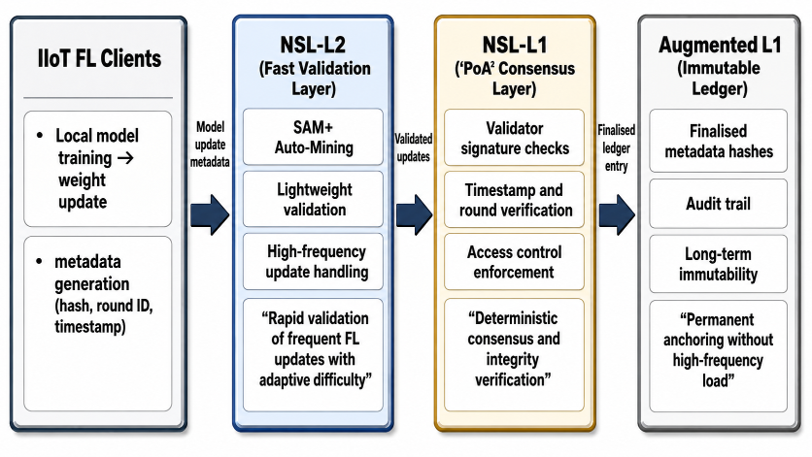
\includegraphics[width=0.95\columnwidth]{figures/Picture9.png}
  \caption{Layered structure of a permissioned industrial ledger, separating the fast layer that records high-frequency operational commitments from the layer that anchors low-frequency, high-value events for external verification.}
  \label{fig:purechain-layers}
\end{figure}

% 

\section{Hybrid Ledger Architectures and Trust Partitioning}
\label{sec:hybrid-ledgers}

From the foregoing analysis, the permissioned ledger of Section~\ref{sec:blockchain-ledgers}, secured by reliability-aware consensus, delivers the fast and deterministic finality that constrained industrial operation requires, but it confines trust to the members of the consortium: an external regulator or partner institution must ultimately take the consortium's word for the integrity of its own records. A single public ledger inverts the problem, offering verification that rests on no single institution while being unable to absorb high-frequency industrial event rates within a realistic device budget. No single ledger satisfies both the speed-and-cost constraint and the external-verifiability constraint at once. Hybrid ledger architectures resolve the tension by combining more than one ledger, and the principle that governs how work is divided between them is trust partitioning: each operation is placed on the layer whose trust model and cost profile match the operation's frequency and value.

\subsection{The Hybrid Ledger Pattern}
\label{subsec:hybrid-pattern}
The hybrid pattern pairs a fast permissioned layer with a public anchoring layer. The permissioned layer records the bulk of operational activity, while the public layer receives only periodic, compact commitments that bind the permissioned state to an externally verifiable record. The scaling literature formalises this as a Layer-1 and Layer-2 relationship, in which a Layer-2 batches many operations and commits a single proof or root to a Layer-1 chain, so that the committed state inherits Layer-1 security at a small fraction of its per-operation cost\cite{rebello2024survey}. The arrangement need not sit within one system: cross-chain and interoperability mechanisms, including relays, notary schemes, and hash-locking, move commitments between heterogeneous ledgers that were never designed to interoperate\cite{hassan2025sok}. Table~\ref{tab:ledger-types} contrasts the public, permissioned, and hybrid options on the properties that decide where an operation belongs.

Across these variants the recurring idea is separation by frequency and value: operations that occur often are kept where they are cheap, and records that must be trusted by outsiders are committed where outsiders can check them. The pattern is therefore defined less by a particular technology than by the placement decision it enforces.

\subsection{Trust Partitioning as an Architectural Principle}
\label{subsec:trust-partitioning}
Read only as a performance optimisation, the fast-plus-anchor split is a caching argument. Read as a trust argument, it is more consequential. The high-frequency behavioural operations of a constrained deployment, such as telemetry, model-update metadata, and intra-consortium validation, carry a trust requirement that the known, vetted validators of a permissioned layer already satisfy, so placing them there sacrifices nothing that an external party needs. The low-frequency, high-value events, such as audit roots, revocation records, and cross-institution commitments, carry a trust requirement that the consortium cannot satisfy on its own account, and only a genuinely public anchor makes them checkable by a party outside the consortium \cite{wang2024public}. Trust partitioning is the discipline of routing each class of event to the layer that can actually vouch for it.

This layered organisation is not merely convenient; layered and tiered blockchain designs have been analysed as a structural response to the resource and trust asymmetries of industrial deployments~\cite{li2025blockchain,song2024novel}, and the structural necessity of such a reference architecture is argued in the systematic review that scaffolds this work (Chapter~\ref{ch:review}). What the principle does not by itself settle is whether a single partitioning rule can hold across different ledger substrates; that question is taken up in Section~\ref{subsec:hybrid-instances}.

\subsection{Instances Across Ledger Substrates}
\label{subsec:hybrid-instances}
The same partitioning principle admits realisations that differ in substrate. Within a single hybrid ledger, a permissioned network-service layering can absorb high-frequency validation while a public augmented Layer-1 preserves the anchored record, so the split is internal to one design. Across two distinct ledgers, a permissioned Hyperledger Fabric network can carry operational transactions while a public Ethereum network holds the anchoring commitments, so the split is a boundary between technologies. Across compute tiers, a federated edge-and-cloud arrangement can partition work by where it is produced and where it must be preserved.

Presented here only as building blocks, these realisations establish three facts: that the pattern exists, that it is a partitioning of trust rather than merely of load, and that more than one substrate can carry it. Whether they express a single, substrate-independent trust-partitioning principle is a question this section deliberately leaves open. Figure~\ref{fig:hybrid-pattern} shows the pattern in its generic form, with a fast permissioned layer feeding periodic commitments to a public anchor.

\begin{table}[t]
  \centering
  \footnotesize
  \setlength{\tabcolsep}{4pt}
  \renewcommand{\arraystretch}{1.25}
  \caption{Public, permissioned, and hybrid ledgers compared on the properties that decide where an operation belongs, after~\cite{al2024shbf}. Entries are inherent properties, not measured results.}
  \label{tab:ledger-types}
  \begin{tabularx}{\columnwidth}{@{}
      >{\raggedright\arraybackslash}p{2.3cm}
      >{\raggedright\arraybackslash}p{2.3cm}
      >{\raggedright\arraybackslash}X
      >{\raggedright\arraybackslash}X@{}}
    \toprule
    \textbf{Ledger type} & \textbf{Write access} & \textbf{Prospects} & \textbf{Limitations} \\
    \midrule
    Public (permissionless) & Open, anonymous & Externally verifiable without a trusted operator; censorship-resistant & Low throughput; probabilistic finality; high cost and energy \\
    \addlinespace
    Permissioned (private / consortium) & Restricted to vetted validators & High throughput; deterministic finality; accountable membership & Trust confined to the operator or consortium; not externally verifiable on its own \\
    \addlinespace
    Hybrid (tiered) & Layered: permissioned plus public & Combines fast permissioned operation with public verifiability; partitions work by frequency and value & Added integration and cross-layer coordination complexity \\
    \bottomrule
  \end{tabularx}
\end{table}



\begin{figure}[t]
  \centering
  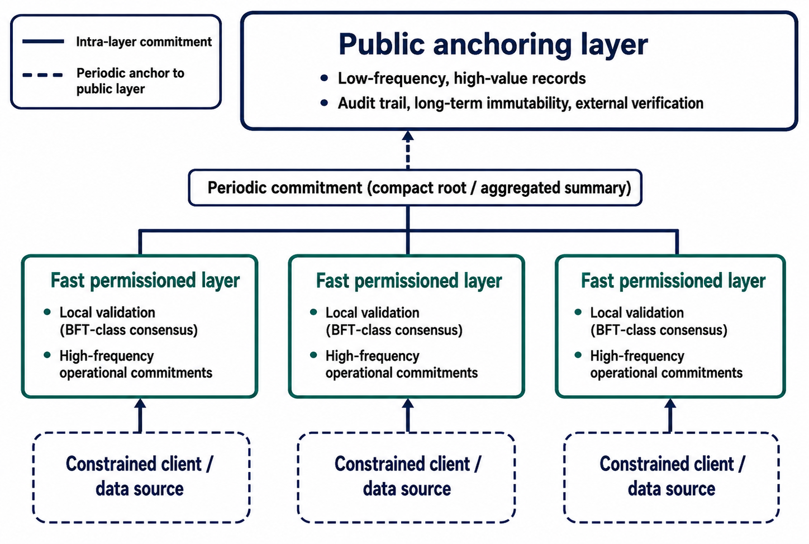
\includegraphics[width=0.99\columnwidth]{figures/Picture10.png}
  \caption{Generic hybrid ledger pattern. Fast permissioned layers absorb high-frequency operational activity and periodically commit a compact root to a public anchoring layer, which preserves low-frequency, high-value records for verification by parties outside the consortium.}
  \label{fig:hybrid-pattern}
\end{figure}



\section{The Case for Trust-Partitioned Security}
\label{sec:case}
Generally, the security of a constrained industrial deployment cannot be delegated to any single mechanism. Section~\ref{sec:bg-landscape} showed that the threat surface is broad and its consequences physical rather than merely informational. Sections~\ref{sec:bg-learning} and~\ref{sec:ai-models} showed that behavioural detection can be made accurate, calibrated, and auditable, but only within a model whose cost and transparency fit the device that must run it. Section~\ref{sec:blockchain-ledgers} showed that a permissioned ledger under reliability-aware consensus can render those decisions tamper-evident at a deterministic and affordable cost. Section~\ref{sec:hybrid-ledgers} showed that a hybrid ledger, governed by trust partitioning, can reconcile the speed a device can afford with the external verifiability a regulator or partner institution demands. Each of these is necessary; none is sufficient on its own.

Read together, they converge on a single requirement: security for constrained, mission-critical IIoT must be at once behavioural, verifiable, and affordable. Behavioural, because static signatures cannot anticipate the attacks that now matter. Verifiable, because a decision that cannot be independently reconstructed cannot be trusted by the parties who bear its consequences. Affordable, because a mechanism that exceeds the device budget is never deployed, whatever its merits on paper. Trust partitioning is the principle that holds these three in tension without sacrificing any of them, by routing each operation to the layer that can both bear its cost and vouch for its trust, so that speed is not bought at the price of verifiability nor verifiability at the price of feasibility.

A fourth requirement is temporal, and it is easily overlooked. The identities and commitments that anchor an industrial system are long-lived: equipment fielded today may still be in service, and still trusted, a decade from now. An adversary therefore need not break current cryptography today, but can record protected traffic now and decrypt it once a cryptographically relevant quantum computer exists, so the effective migration deadline is set by the lifetime of the data rather than by the arrival of the machine \cite{singh2024managing}. The standardisation of post-quantum key encapsulation and signatures, noted in Section~\ref{sec:bg-landscape}, makes migration possible; what makes it hard is that lattice-based schemes carry larger keys and ciphertexts than the elliptic-curve schemes they replace, pressing on exactly the memory and transmission budgets that already constrain these devices \cite{castiglione2024integrating}. Post-quantum resistance is thus not a separate concern bolted onto the architecture but another face of the same affordability problem: the cryptographic anchor of trust must be quantum-resistant and compact at once.

Beneath all four requirements runs the resource budget, which is less a requirement than a filter applied to every other choice. It is the budget that rules out proof-of-work, that forbids unbounded validator sets, that penalises opaque high-capacity models, and that turns post-quantum migration from a configuration change into a design problem. A proposal that sets the budget aside is not conservative but inapplicable, and much of the apparent disagreement across the mechanisms surveyed here dissolves once the budget is treated as binding rather than negotiable.

Taken together, these requirements describe a target that none of the mechanisms in isolation reaches: a security architecture that is behavioural in its detection, tamper-evident in its record, trust-partitioned in its structure, post-quantum in its cryptographic anchor, and viable within a real device budget throughout. The case for trust-partitioned security is the case that these properties are jointly necessary and jointly attainable, rather than a menu from which one selects. Whether existing practice already offers such an architecture, and if it does not, precisely where and why it falls short, cannot be settled from the selective reading of a background chapter. It calls for the systematic, reproducible review undertaken in Chapter~\ref{ch:review}, where the distance between these requirements and what current approaches deliver is measured and the resulting gap made precise.